\documentclass[tikz]{standalone}
\usepackage{amsmath,amssymb}

\newcommand{\twovec}[2]{\ensuremath{\begin{pmatrix}{#1}\\{#2}\end{pmatrix}}}
\NewCommandCopy{\oldvec}{\vec} % https://tex.stackexchange.com/questions/47351/can-i-redefine-a-command-to-contain-itself
\renewcommand{\vec}[1]{\oldvec{\mathbf{#1}}}

% Hexagonal lattice
\newcommand{\onex}{0.8}
\newcommand{\twox}{0.3}\newcommand{\twoy}{0.9}

\begin{document}
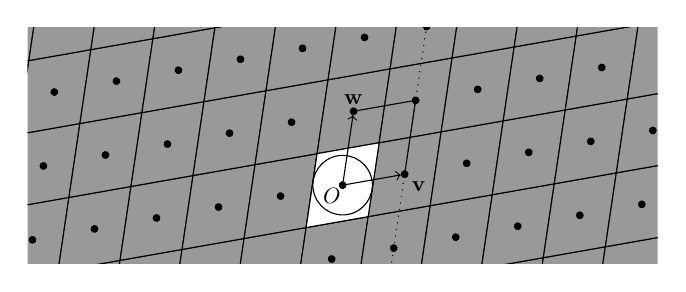
\begin{tikzpicture}
	\clip (-4, -1) rectangle (4,2);
	\tikzset{every node/.style={inner sep=3pt,scale=0.8}}

	\begin{scope}[rotate=10]
		% Lattice with basis [(\onex,0), (\twox,\twoy)]
		\foreach\one in {-6,-5,...,6}{\foreach\two in {-2,-1,0,1,2,3}{%
			\draw[draw=black,fill=black!40!white]
				({\onex*(\one-.5) + \twox*(\two-.5)},{\twoy*(\two-.5)}) --
				({\onex*(\one+.5) + \twox*(\two-.5)},{\twoy*(\two-.5)}) --
				({\onex*(\one+.5) + \twox*(\two+.5)},{\twoy*(\two+.5)}) --
				({\onex*(\one-.5) + \twox*(\two+.5)},{\twoy*(\two+.5)}) -- cycle;
			\fill[black] (\one*\onex + \two*\twox, \two*\twoy) circle (.05);
		}}

		\draw[draw=black,fill=white]
			({\onex*(-.5) + \twox*(-.5)},{\twoy*(-.5)}) --
			({\onex*(+.5) + \twox*(-.5)},{\twoy*(-.5)}) --
			({\onex*(+.5) + \twox*(+.5)},{\twoy*(+.5)}) --
			({\onex*(-.5) + \twox*(+.5)},{\twoy*(+.5)}) -- cycle;

		\draw[dotted] (\onex - 10*\twox, -10*\twoy) -- (\onex + 10*\twox, 10*\twoy);

		\draw[draw=none,fill=black] (0,0) circle (.05);

		\draw (0,0) circle (\onex/2*0.9449);

		\node[anchor=north east,circle,inner sep=1pt] at (0,0) {\(O\)};
		\draw[shorten >=1.4pt,->] (0,0) -- (\onex,0) node[below right] {\(\vec{v}\)};
		\draw[shorten >=1.4pt,->] (0,0) -- (\twox,\twoy) node[above] {\(\vec{w}\)};
		\draw[shorten >=1.4pt] (\onex,0) -- (\onex + \twox,\twoy);
		\draw[shorten >=1.4pt] (\twox,\twoy) -- (\onex + \twox,\twoy);
	\end{scope}
\end{tikzpicture}
\end{document}
